\chapter{Учебные примеры}
\label{chap:2}
В этой главе мы опишем подробно процесс установки, моделирования и пост- процесорной обработки для некоторых тестовых
 примеров OpenFOAM, с основной целью: познакомить пользователя с основными процедурами работы и управления OpenFOAM.
 \textit{\$FOAM\_TUTORIALS} директория содержит много тестовых случаев, которые демонстрируют использование всех
 решателей и многих утилит поставляемых с OpenFOAM. Прежде чем пытаться использовать обучающие программы, пользователь
 должен предварительно удостовериться  в том, что он установил OpenFOAM правильно.

Обучающие примеры описывают использование утилиты \textsl{blockMesh} - инструмента предпроцессорной обработки, установки 
примера и запуска на счет решателя OpenFOAM и постпроцессорной обработки с использованием \textsl{paraFoam}.
 Те пользователи, которые имеют доступ к постпроцессорам, разработанным другими фирмами (из инструментария посторонних
 разработчиков), также поддерживаемых в OpenFOAM, имеют выбор: либо они могут следовать за примерами обучающих программ,
 используя \textsl{paraFoam}; либо обратиться к описанию использования продукта постороннего разработчика, как описано в
\autoref{chap:6}, когда требуется постпроцессорная обработка.

Копии всех обучающих программ доступны в директории \textit{tutorials} из поставки OpenFOAM.
Обучающие программы организованы
 в виде ряда директорий согласно типу течения в которых расположены поддиректории согласно решателю. Например,
 все \textsl{icoFoam} примеры хранятся в пределах подкаталога
 \textit{incompressible/icoFoam}, где \textit{incompressible}
(несжимаемое)  указывает на тип рассматривваемого течения. Если пользователь желает запустить на расчет несколькотестовых 
примеров,  рекомендуется, чтобы пользователь сначала скопировал директорию \textit{tutorials} в свою локальноую директорию
\textit{run}. Они могут быть легко скопированы набором:

\texttt{mkdir –p \$FOAM\_RUN}

\texttt{cp –r \$FOAM\_TUTORIALS \$FOAM\_RUN}

\section{Течение в прямоугольной полости, инициированное верхней плитой}
\label{sec:2.1}
Этот раздел руководства описывает как выполнить этапы пре-процессор, расчет и постпроцессорную обработку для тестового
 примера, рассматривающего изотермическое течение несжимаемой среды в двумерной квадратной области. Геометрия течения
изображена на Рис. 2.1, в которой все границы квадрата являются стенками. Верхняя стенка перемещается в
\textit{x}-направлении со скоростью 1 м/с, в то время как другие 3 неподвижны. Первоначально принято, что будет
 рассматриваться ламинарное течение и задача будет решаться на однородной сетке, используя решатель \textsl{icoFoam}
 для ламинарного, изотермического, несжимаемого потока. В течение курса обучающей программы, будут исследованы влияние
 увеличения числа узлов сетки на решение и влияние измельчения шага сетки по направлению к стенкам.
Наконец, число Рейнольдса будет увеличено, и решатель \textsl{pisoFoam} будет использоваться для турбулентного,
 изотермического, несжимаемого течения.

\begin{figure}[h]
 \centering
 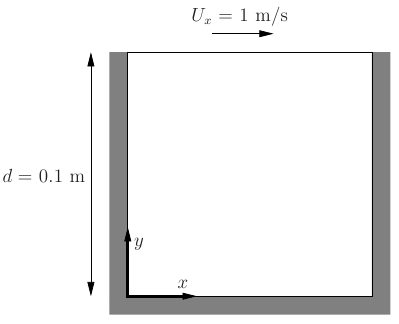
\includegraphics[width=299pt,height=243pt]{UGFigure2-1.PNG}
 % UGFigure2-1.PNG: 399x324 pixel, 96dpi, 10.56x8.57 cm, bb=0 0 299 243
 \caption{Геометрия течения в каверне, инициированного движением верхней плиты.}
 \label{fig:2.1}
\end{figure}

\section{Пре- процессорная подготовка (pre-processing)}
\label{sec:2.1.1}

В составе дистрибутива OpenFOAM поставляются примеры. Для редактирования файлов примера пользователь должен выбрать
 xeditor или другой редактор , типа \textbf{emacs}, \textbf{vi}, \textbf{gedit}, \textbf{kate}, \textbf{nedit},
 и т.п. Редактирование файлов возможно в OpenFOAM, потому что ввод / вывод использует формат словаря с ключевыми
 словами, которые представляют смысловое значение, чтобы быть понятными даже наименее опытным пользователям.

Моделируемый случай включает данные для сетки, полей, свойств, параметров контроля решения, и т.д.
 Как описано в секции 4.1, в OpenFOAM эти данные хранятся в ряде файлов в пределах директории примера,
 а не в единственном файле примера, как во многих других пакетах вычислительной гидродинамики (CFD).
 Директории примера дают соответственно описательное название, например первый случай для этого
 обучающего примера просто назван \textsl{cavity} (каверна). В подготовке редактирования файлов примера и
 запуска первого примера \textsl{cavity}, пользователь должен перейти в каталог примера

\texttt{cd \$FOAM\_RUN/tutorials/incompressible/icoFoam/cavity}

\subsection{Генерация сетки}
\label{sec:2.1.1.1}

OpenFOAM всегда работает в 3 мерной декартовой системе координат и все геометрические конфигурации производятся
 в 3 измерениях. OpenFOAM решает примеры в 3 измерениях по умолчанию, но может быть проинструктирован решать
 в 2 измерениях, определяя специальное \textsl{empty} (пустое) граничное условие на границах, нормальных к (3-ему)
 z измерению (для данного примера), для которого никакое решение проводить не требуется.
Область примера \textsl{cavity} состоит из квадрата c длинами сторон \textit{d} = 0.1 м. в \textit{x-y} плоскости.
Первоначально будет использоваться равномерная сетка 20 на 20 ячеек. В блочной конструкции показанной на \autoref{fig:2.2}. генератор сеток,
 поставляемый с OpenFOAM, \textit{blockMesh}, создает сетки, используя команды из описания определенного в словаре ввода,
 \textit{blockMeshDict} расположенного в каталоге \textit{constant/polyMesh} данного примера. Чтобы перейти к
 \textit{blockMeshDict}  для этого примера  возьмем следующий файл:
\begin{verbatim}
/*--------------------------------*- C++ -*----------------------------------*\
| =========                 |                                                 |
| \\      /  F ield         | OpenFOAM: The Open Source CFD Toolbox           |
|  \\    /   O peration     | Version:  2.1.0                                 |
|   \\  /    A nd           | Web:      www.OpenFOAM.com                      |
|    \\/     M anipulation  |                                                 |
\*---------------------------------------------------------------------------*/
FoamFile
{
    version     2.0;
\end{verbatim} 

\begin{figure}[ht]
 \centering
 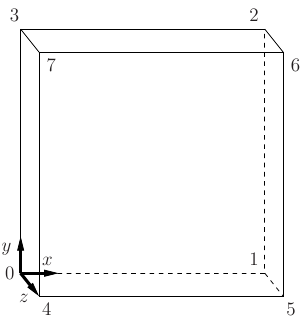
\includegraphics[width=229pt,height=241pt]{UGFigure2-2.PNG}
 % UGFigure2-2.PNG: 306x321 pixel, 96dpi, 8.10x8.49 cm, bb=0 0 229 241
 \caption{Блочная конструкция сетки для каверны.}
 \label{fig:2.2}
\end{figure}

\begin{verbatim}
    format      ascii;
    class       dictionary;
    object      blockMeshDict;
}
// * * * * * * * * * * * * * * * * * * * * * * * * * * * * * * * * * * * * * //

convertToMeters 0.1;

vertices        
(
    (0 0 0)
    (1 0 0)
    (1 1 0)
    (0 1 0)
    (0 0 0.1)
    (1 0 0.1)
    (1 1 0.1)
    (0 1 0.1)
);

blocks          
(
    hex (0 1 2 3 4 5 6 7) (20 20 1) simpleGrading (1 1 1)
);

edges           
(
);

boundary
(
    movingWall 
    {
        type wall;
        faces
        (
            (3 7 6 2)
        );
    }
    fixedWalls 
    {
        type wall;
        faces
        (
            (0 4 7 3)
            (2 6 5 1)
            (1 5 4 0)
        );
    }
    frontAndBack 
    {
        type empty;
        faces
        (
            (0 3 2 1)
            (4 5 6 7)
        );
    }
);

mergePatchPairs 
(
);

// ************************************************************************* //

\end{verbatim}

В начале файла содержится заголовок в форме баннера (строки 1-7), далее информация файла
 содержится в подсловаре \textsl{FoamFile}, заключенная в фигурных скобках (\verb|{|\ldots\verb|}|).

\textit{В остальной части руководства:}
Ради сохранения места и для ясности, шапка или заголовок файла, включая баннер и \textsl{FoamFile} подсловарь,
 и обрамление в скобках не будут включаться в файлы примеров.

Файл в начале содержит блок вершин \texttt{vertices} (x,y,z координаты точек); затем в нем определяются сами блоки
 (\texttt{blocks})  (в данном примере имеется только 1) с помощью описанных выше меток вершин и номеров
 ячеек внутри них; и наконец, в файле определяются поверхности для задания граничных патчей.
 Пользователю предлагается обратиться к \autoref{sec:5.3} чтобы понять значение вводимых  величин в \textsl{blockMeshDict} файле.

Сетка генерируется при запуске утилиты \textsl{blockMesh}, использующей файл \textsl{blockMeshDict}.
Запуск производится из директории задачи, просто набором команды в терминале:

\texttt{blockMesh}

Состояние выполнения \textsl{blockMesh} выводится в окне терминала. Любые ошибки в исходном 
файле сетки \textsl{blockMeshDict} обрабатываются textsl{blockMesh} и итоговые сообщения об ошибках показывают 
пользователю номер строки в которой возникла проблема. На этой стадии не должно быть никаких сообщений об ошибках.

\subsection{Граничные и начальные условия}
\label{sssec:2.1.1.2}

Как только генерация сетки окончена, пользователь может посмотреть на заданные начальные поля установленные для этого
 расчетного случая. Пример установлен на начальное время t = 0 сек, так что данные о начальных полях
 хранятся в поддиректории \textit{0} каталога примера \textit{cavity}. Поддиректория \textit{0} содержит
 2 файла, \textit{p} и \textit{U}, по одному для полей давления (p) и скорости (U),
 чьи начальные значения и граничные условия должны быть заданы. Давайте проверим файл давления \textit{p}:

\begin{verbatim}
dimensions      [0 2 -2 0 0 0 0];

internalField   uniform 0;

boundaryField
{
    movingWall      
    {
        type            zeroGradient;
    }

    fixedWalls      
    {
        type            zeroGradient;
    }

    frontAndBack    
    {
        type            empty;
    }
}

// ************************************************************************* // 
\end{verbatim} 

Сущестуют 3 главных раздела ввода полей данных файлов:

\texttt{dimensions} (размерности) определяют величину размерности поля, здесь \textit{кинематическое}
 давление, $m^2 s^{−2}$ (баротропия или отношение давления к плотности => (N/$m^2$) /(кг/$m^3$)=$m^2$/$s^2$)
 (смотрите \autoref{ssec:4.2.6} для более детальной информацией);

\texttt{internalField} данные поля внутри расчетной области, которое может быть задано однородным (\texttt{uniform}),
 описываемым одной цифровой величиной; или неоднородным (\texttt{nonuniform}), где все значения поля должны быть заданы
 (смотрите \autoref{ssec:4.2.8} для более подробной информацией);

\texttt{boundaryField} данные о граничных полях, которые включают граничные условия, и данные обо всех граничных
 патчах (boundary patches) (смотрите \autoref{ssec:4.2.8} для более подробной информации).

Для данного примера каверны (\textsl{cavity}), границы состоят только из стенок, разбитые на 2 патча
 названных: (1) \textsl{fixedWall} для неподвижных фиксированных боковых стенок и основания каверны; (2) \textsl{movingWall}
для подвижного верха каверны. На стенках, и тех и других, граничное условие для давления \textsl{p} есть \textsl{zeroGradient},
 что означает “нормальный градиент давления равен нулю”. Патчи \textsl{frontAndBack} представляют переднюю и заднюю
 плоскости и поэтому для двумерного случая должны быть заданы \textsl{empty} (пустой).

В этом примере, как и в большинстве с которыми мы встретились, начальные поля заданы однородными (uniform).
 Здесь давление является кинематическим, и как для несжимаемой среды, абсолютное значение
 его не имеет значения (во всех уравнениях нет самого давления а только его производные), поэтому оно
 задается как \texttt{uniform 0} для удобства.

Пользователь может аналогично проверить поле скорости в файле \textsl{0/U}. Размерности \textsl{dimensions}
 необходимы для скорости, внутреннее поле инициализируется как одногродное нулевое \textsl{uniform zero},
 что в случае скорости должно быть представлено тремя компонентами, т.е. \textsl{uniform (0 0 0)} (смотри
 \autoref{ssec:4.2.5} для более подробной информации).

Граничные условия для скорости требуют аналогичных граничных условий (empty) для переднего
 и заднего патчей \textsl{frontAndBack}. Другими патчи являются стенками (walls): условие
 непроскальзывания (no-slip) задаётся на поверхностях \textsl{fixedWalls}, следовательно
 условие \textsl{$fixedValue$} со значением \texttt{uniform (0 0 0)}. Верхняя поверхность движется
 со скоростью 1 м/с в направлении оси \textit{x}, что тоже требует условия \textsl{fixedValue}, но со значением 
\texttt{uniform (1 0 0)}.

\subsection{Физические свойства}
\label{sssec:2.1.1.3}

Физические свойства для кейса хранятся в словарях (dictionaries), к чьим именам добавляются суффиксы 
\textsl{...Properties} (Свойства), расположены в дереве каталогов \textit{Dictionaries}.
 Для кейса \textsl{icoFoam}, должно быть задано единственное свойство это кинематическая вязкость, которая хранится
 в словаре \textit{transportProperties}. Пользователь может проверить, что кинематическая вязкость
 задана правильно открыв словарь \textit{transportProperties} а также просмотреть/отредактировать его содержимое.
 Ключевое слово для кинематической вязкости \textsl{nu}, фонетическое обозначение
 греческой буквы $\nu$ которой вязкость обозначена в уравнениях. Первоначально этот кейс будет запущен с числом Рейнольдса
равным $10$, где число Рейнольдса определяется как:
\begin{equation}
 Re = \frac{d|\bf U|}{\nu}
 \label{eq:2.1}
\end{equation}

где $d$ и $\bf{U}$ характеристики размер и модуль скорости соответственно, а $\nu$ кинематическая вязкость.
 В примере $d = 0.1 m$, $|\bf U| = 1 ms^{−1}$, так что для $Re = 10$, $\nu = 0.01{m^{2}s^{-1}}$.

Верными входными величинами для кинематической вязкости являются представленные ниже значения:

\begin{verbatim}[file, linenum=17]

nu              [0 2 -1 0 0 0 0] 0.01;


// ************************************************************************* //
\end{verbatim} 

\subsection{Управление}
\label{sssec:2.1.1.4}

Входные данные, относящиеся к управлению временем чтения и записи данных решения находятся в \textit{controlDict}. 
Пользователь должен просмотреть данный файл, так как это основной файл управления, находится в папке \textit{system}.

Для запуска необходимо задать время начала и конца решения, а также шаг по времени. OpenFOAM предоставляет 
широкие возможности по управлению временем. Подробное описание вы найдете в \autoref{sec:4.3}. В этом руководстве
 мы хотим начать запуск в момент времени  $t = 0$, это значит что OpenFOAM необходимо считать данные из каталога
 $0$ (см. \autoref{sec:4.1}). Поэтому мы задаем значения для \texttt{startFrom} и \texttt{startTime}, а затем назначаем
 \texttt{startTime} значение $0$.

Для конечного шага по времени мы хотим получить стационарное решение для потока, циркулирующего внутри полости каверны.
 Как правило жидкость должна пройти через объем 10 раз прежде чем достичь состояния устойчивого ламинарного течения. 
В данном случае поток не проходит сквозь объем, так как здесь нет ни входа ни выхода,
 поэтому в качестве конечного момента времени расчета может быть задано время, требующееся на то, чтобы крышка проехала
 через каверну десять раз, т.е. 1 с; по предыдущим расчетам видим, что достаточно и 0.5 с, поэтому будем использовать
 это значение. Чтобы задать это конечное время дадим параметру \texttt{stopAt} значение \texttt{EndTime},
 а затем установим для параметра \texttt{EndTime} значение 0.5.

Теперь необходимо установить шаг по времени, который задется параметром \texttt{deltaT}. 
Для достижения  точности по времени и численной стабильности при запуске icoFoam,
 необходимо число Куранта меньше 1. Число Куранта для одной ячейки определяется как:
\begin{equation}
 C_o = \frac{\delta t|\bf U|}{\delta x}
\end{equation}
где $\delta t$ это шаг по времени, $|\bf U|$ это величина скорости через эту ячейку и $\delta x$ размер ячейки 
по направлению скорости. Скорость потока непостоянна в пределах области, но условие
 $C_o<1$ должно выполняться во всей области. Поэтому мы выберем $\delta t$ на основе наихудшего варианта:
 \textit{максимальное} значение $C_o<1$ соответствовует совокупности большой величины скорости
 течения и малого размера ячейки. В нашем случае размер ячейки в области постоянный,
 поэтому максимальное значение $C_o<1$ будет вблизи двигающейся крышки, где скорость около 1 м/с.
 Соответственно размер ячейки определяется по формуле:
\begin{equation}
 \delta x = \frac{d}{n} = \frac{0.1}{20} = 0.005 m
\end{equation}
Следовательно чтобы получить число Куранта меньше или равное 1 во всей области, шаг по времени \texttt{deltaT}
 должен быть меньше или равен:
\begin{equation}
 \delta x = \frac{C_o \delta x}{|\bf U|} = \frac{1 \times 0.005}{1} = 0.005 s
\end{equation}
В процессе моделирования мы решили записывать результаты через определенные промежутки времени,
 что мы можем позднее просмотреть с помощью постпроцессора. Оператор \texttt{writeControl} предоставяет несколько
 опций для настройке моментов времени, в которые будут записываться результаты; здесь мы выбираем опцию \texttt{timeStep},
 которая задает, что результаты будут записываться каждый \textit{n}-ый шаг по времени,
 где значение \textit{n} задается параметром \texttt{writeInterval}. Допустим мы хотим записывать
 результаты в моменты 0.1, 0.2, . . . , 0.5 с - с шагом 0.005 с, для этого необходимо выводить результаты на каждом
 20-ом шаге, поэтому мы установили значение \texttt{writeInterval} равное 20.

OpenFOAM создает новую папку с \textit{именем соответсвующего момента времени}, например, 0.1 с. И каждый раз,
 записывается набор данных, что более подробно описано в разделе 4.1.
 В решателе \textsl{icoFoam} во временные каталоги записываются значения полей \texttt{U} и \texttt{p}.
 Для нашего примера, содержание \textit{controlDict} приведено ниже:

\begin{verbatim}
application     pisoFoam;

startFrom       startTime;

startTime       0;

stopAt          endTime;

endTime         0.5;

deltaT          0.005;

writeControl    timeStep;

writeInterval   20;

purgeWrite      0;

writeFormat     ascii;

writePrecision  6;

writeCompression off;

timeFormat      general;

timePrecision   6;

runTimeModifiable true;

// ************************************************************************* //
\end{verbatim}

\subsection{Дискретизация и параметры решателя}
\label{sec:2.1.1.5}

Пользователь указывает выбранные схемы конечно-элементной дискретизации в файле \textit{fvSchemes}
 директории \textit{system}. Описание решателей систем линейных уравнений, задание точности и настройка алгоритмов
 происходит в файле \textit{fvSolution} той же директории \textit{system}. Пользователь может просмотреть все
 эти файлы, но мы пока не будем подробно описывать их содержимое, за исключением параметров \texttt{pRefCell}
 и \texttt{pRefValue} в \textit{PISO} - подсловаре \textit{fvSolution}. В закрытой несжимаемой системе,
 такой как каверна, давление относительное: в диапазоне давлений значения не абсолютные.
 В таких случаях в решателе задается исходный уровень с помощью опции \texttt{pRefValue} в ячейке \texttt{pRefCell}.
 В нашем примере оба значения равны 0. Изменение любого из этих
 значений повлияет на абсолютное значение давления, но не на относительные значения скорости или давления.

\section{Просмотр сетки}
\label{sec:2.1.2}

Проверить сетку на наличие ошибок перед запуском - хорошая идея.
 Сетку можно просмотреть в \textsl{paraFoam}, постпроцессоре, распространяемом вместе с OpenFOAM.
 Постпроцессор \textsl{paraFoam} можно запустить набрав в терминале следующую команду из каталога проекта 

\texttt{paraFoam}

Также он может быть запущен из любой другой директории если добавлена опция \texttt{-case} аргументом которой является
путь к проекту, например

\texttt{paraFoam -case \$FOAM\_RUN/tutorials/incompressible/icoFoam/cavity}

Эта команда запускает окно \textsl{ParaView} как показано на рисунке 6.1. В \textsl{Pipeline Browser},
 пользователь может видеть, что в \textsl{ParaView} открыт файл \textsl{cavity.OpenFOAM},
 для \textsl{cavity}. Перед нажатием на кнопку \textsl{Apply} (Применить),
 пользователю нужно выбрать геометрию в панели \textsl{Mesh Parts}. Так как проект небольшой, то самое простое - выбрать
 все компоненты в заголовке панели \textsl{Mesh Parts}. Пользователю необходимо нажать кнопку \textsl{Apply} (Применить)
для начала загрузки геометрии в \textsl{ParaView}.

Откройте панель \textsl{Display}, которая отвечает за визуализацию выбранного модуля. В панели \textsl{Display} выполните 
следующие действия, как показано на рисунке 2.3: (1) установите Цвет по \textsl{Solid Color},
 (2) нажмите \textsl{Set Solid Color} и выберите подходящий цвет, например черный (для белого фона);
 (3) в панели \textsl{Style} выберите \textsl{Wireframe} в меню Representation.
 Цвет фона можно задать, выбрав \textsl{View Settings} в меню \textsl{Edit} на строке меню вверху.

Особенно если вы впервые пользуетесь ParaView, мы рекомендуем вам работать с изображением, как описано в разделе 6.1.5.
 В частности, поскольку это двумерная модель, рекомендуем вам выбрать Use Parallel Projection
 в панели General настройки окна выбранного в меню Edit. Ориентацию осей можно включить или выключить
 в окне Annotation, также положение переключателя можно изменять при помощи мыши.

\section{Запуск приложения}
\label{sec:2.1.3}

Как и любые исполняемые Unix/Linux приложения, OpenFOAM можно запустить двумя способами: как главный процесс, т.е. в котором оболочка ждет завершения выполнения команды, прежде чем запустить командную строку; и как фоновый процесс, который в течение процесса выполнения позволяет вызвавшей оболочке получать дополнительные команды. 
В данном случае мы будем запускать icoFoam в качестве главного процесса. Солвер icoFoam выполняется либо путем ввода в каталоге, набрав

\begin{verbatim}
icoFoam 
\end{verbatim}

в командной строке, либо с помощью -case с выборочным параметром,зависящим от каталога, например:

\begin{verbatim}
icoFoam -case $FOAM RUN/tutorials/incompressible/icoFoam/cavity
\end{verbatim}

Ход решения записывается в окне терминала. Он сообщает пользователю текущее время, максимальное значение числа Куранта, начальные и конечные невязки решения по всем направлениям течения.

\section{Последующая обработка (Post-processing)}
\label{sec:2.1.4}

В то время как результаты записываются во временные каталоги, их можно просмотреть с помощью paraFoam. Вернитесь к окну paraFoam и выберите панель Properties для cavity.OpenFOAM модуля. Если нужное окно панелей в случае модуля, не отображается в любой момент времени, пожалуйста, убедитесь, что: cavity.OpenFOAM подсвечивается синим цветом, а кнопка (глаза) eye рядом с ним нажата и показывает, что графика включена;
Чтобы подготовить paraFoam для отображения данных, представляющих интерес, мы должны сначала загрузить данные в соответствующий момент времени 0,5 сек. Если процесс был запущен в то время как ParaView был открыт, выходные данные во временных директориях не будут автоматически загружаться в среду ParaView. Для загрузки данных пользователь должен выбрать Update GUI в окне Properties, а затем нажать зеленую кнопку Apply. Временные данные будут загружены в ParaView.

\begin{figure}[ht]
%  \centering
%  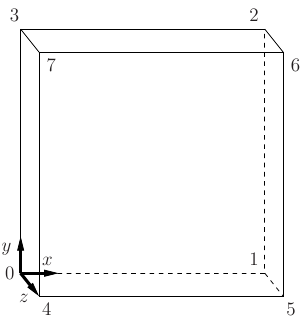
\includegraphics[width=229pt,height=241pt]{UGFigure2-2.PNG}
%  % UGFigure2-2.PNG: 306x321 pixel, 96dpi, 8.10x8.49 cm, bb=0 0 229 241
%  \caption{Показаны характеристики давления для каверны.}
%  \label{fig:2.2}
\end{figure}

\begin{figure}[ht]
%  \centering
%  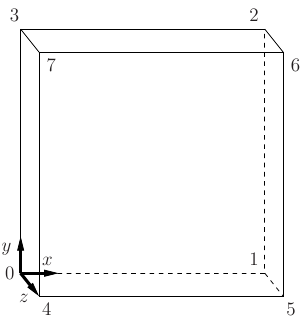
\includegraphics[width=229pt,height=241pt]{UGFigure2-2.PNG}
%  % UGFigure2-2.PNG: 306x321 pixel, 96dpi, 8.10x8.49 cm, bb=0 0 229 241
%  \caption{Распределение давлений для модели каверны.}
%  \label{fig:2.2}
\end{figure}

\section{Поверхности постоянных значений и профильные диаграммы (Isosurface and contour plots)}
\label{sec:2.1.4.1}
